\documentclass{article}

% if you need to pass options to natbib, use, e.g.:
\PassOptionsToPackage{numbers, compress}{natbib}
% before loading neurips_2024


% ready for submission
\usepackage{neurips_2024}


% to compile a preprint version, e.g., for submission to arXiv, add add the
% [preprint] option:
    % \usepackage[preprint]{neurips_2024}


% to compile a camera-ready version, add the [final] option, e.g.:
    % \usepackage[final]{neurips_2024}


% to avoid loading the natbib package, add option nonatbib:
    % \usepackage[nonatbib]{neurips_2024}


\usepackage[utf8]{inputenc} % allow utf-8 input
\usepackage[T1]{fontenc}    % use 8-bit T1 fonts
\usepackage{hyperref}       % hyperlinks
\usepackage{url}            % simple URL typesetting
\usepackage{booktabs}       % professional-quality tables
\usepackage{amsfonts}       % blackboard math symbols
\usepackage{nicefrac}       % compact symbols for 1/2, etc.
\usepackage{microtype}      % microtypography
\usepackage{xcolor}         % colors
\usepackage{graphicx}       % include graphics


\title{First Paper Summary, EE245 Spring 2025}

\begin{document}

% pdflatex main.tex; bibtex main; pdflatex main.tex; pdflatex main.tex

\maketitle

\begin{abstract}
  The first paper summary due on Monday, Apr. 28, 2025. The author chose the paper titled "\underline{Mastering Diverse Domains through World Models}" by Danijar Hafner, Jurgis Pasukonis, Jimmy Ba, and Timothy Lillicrap.

  The following content covers 1) major contributions, 2) prior work, 3) method, 4) major results, 5) strengths, and 6) weaknesses.
\end{abstract}

% Components (2-3 pages)
% 1. Summary of major contributions – 15%
% 2. Relation to prior work – 15%
% 3. Summary of the method – 20%
% 4. Summary of major results – 20%
% 5. Summary of strengths – 15%
% 6. Summary of weaknesses – 15%

\section{Summary of Major Contributions}

The main contribution of this paper \cite{hafner2023mastering} is the introduction of a general reinforcement learning algorithm called Dreamer (specifically, DreamerV3), which contains a world model, a critic neural network (NN), and a actor NN. Dreamer masters a wide range of domains (over 150 tasks) with fixed hyperparameters. Furthermore, the algorithm can learn robustly across different data and compute budgets, making it applicable to a variety of practical applications. It overcomes the challenges of robustly learning through techniques based on normalization, balancing, and transformations.

The paper conducts comprehensive experiments to evaluate the performance of Dreamer across different environments, including Minecraft, Atari, ProcGen, and others. In the task of Minecraft, Dreamer is the first algorithm to collect diamonds from scratch while keeping configurations the same. The algorithm shows the ability to learn farsighted strategies from pixels and sparse rewards in an open world.

Dreamer paves the way for future research directions, including teaching agents world knowledge from internet videos and learning a single world model across domains. This allows artificial agents to build up increasingly general knowledge and competency.

\section{Relation to Prior Work}

Plenty of prior work has been done in the field of general-purpose reinforcement learning algorithms, such as PPO \cite{schulman2017proximal}, SAC \cite{haarnoja2018soft}, MuZero \cite{schrittwieser2020mastering}, and Gato \cite{reed2022generalist}. However, these algorithms face challenges in lower performance, requirements for tuning, no open-source code, or demanding expert data. Dreamer, on the other hand, ``masters a diverse range of environments with fixed hyperparameters, does not require expert data, and its implementation is open source'' \cite{hafner2023mastering}.

Besides over 150 tasks conducted in the paper, Dreamer demonstrates its outstanding performance in the Minecraft environment, MALMO (Microsoft version) \cite{johnson2016malmo} and MineRL (experiments used version) \cite{milani2020minerl}. Prvious methods like Voyager \cite{wang2023voyager} and VPT \cite{baker2022video} indeed show impressive performance in Minecraft, but they require specifically engineered or hundreds of computational resources. In contrast, Dreamer autonomously learns to collect diamonds within very limited resources and without human data.

\section{Summary of the Method}

The third generation of Dreamer is a model-based, online, general-purpose reinforcement learning algorithm. The algorithm has three NNs: a world model, a critic, and an actor. All the three NNs are trained concurrently from replayed experience. The figure below shows the architecture of DreamerV3 are copied from the paper:

\begin{figure}[h]
    \centering
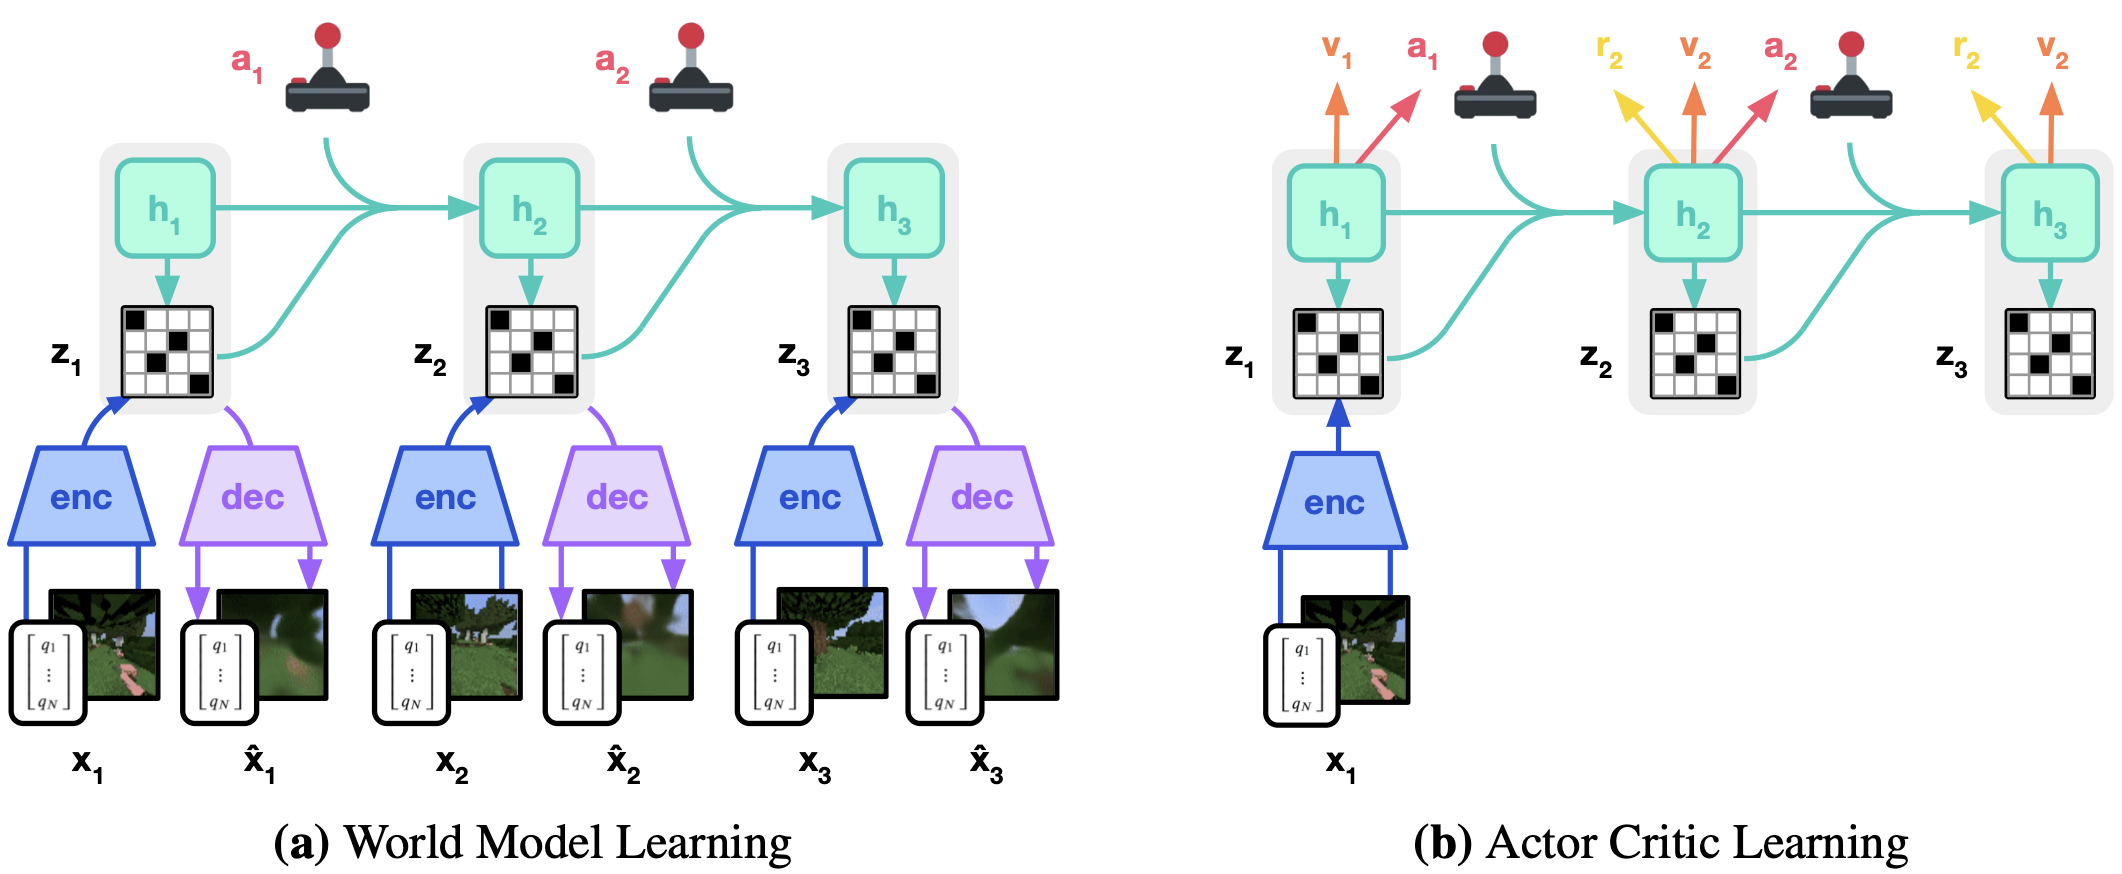
\includegraphics[width=0.7\textwidth]{./pics/learnings.png}
    \caption{Architecture of DreamerV3 \cite{hafner2023mastering}}
    \label{fig:architecture}
\end{figure}

\textbf{World model learning} is responsible for learning the dynamics of the environment by predicting future representations and rewards for potential actions. The paper implement a Recurrent State-Space Model (RSSM) to learn the world model. Given a batch of inputs, actions, rewards, and continuations flags, the world model are optimized by minimizing the three losses by weights: prediction loss $\beta_{pred}\mathcal{L}_{pred}$, dynamics loss $\beta_{dyn}\mathcal{L}_{dyn}$, and representation loss $\beta_{rep}\mathcal{L}_{rep}$. These losses allows world model with fixed hyperparameters to fit across domains.

\textbf{Actor Critic learning} are conducted entirely within the latent space using abstract trajectories predicted by the world model. The actor and critic operate on model states $s_t \doteq \{h_t, z_t\}$. For each model state, the actor network $a_t \sim \pi_\theta(a_t | s_t)$ aims to maximize the discount return $R_t \doteq \sum_{\tau = 1}^{\infty} \gamma^{\tau} r_{t+\tau}$ with discount factor $\gamma = 0.997$. Meanwhile, the critic network $v_\psi(R_t | s_t)$ estimates the state-value function for each state under the current policy, which can approximate the $\gamma$-reward over prediction horizon $T=16$. The customized A-C framework make DreamerV3 more efficient and robust.

\section{Summary of Major Results}

The paper conducts comprehensive experiments to evaluate the performance of DreamerV3 across 8 domains -- over 150 tasks -- using the same hyperparameters. PPO \cite{schulman2017proximal} is used as the baseline compared to DreamerV3 and other SOTA algorithms. Noticeably, DreamerV3 also runs on the challenging Minecraft environment. All the experiments are conducted on a single NVIDIA A100 GPU, and the code and results are open-sourced. A summary of the results from the paper is shown in the figure below:

\begin{figure}[h]
    \centering
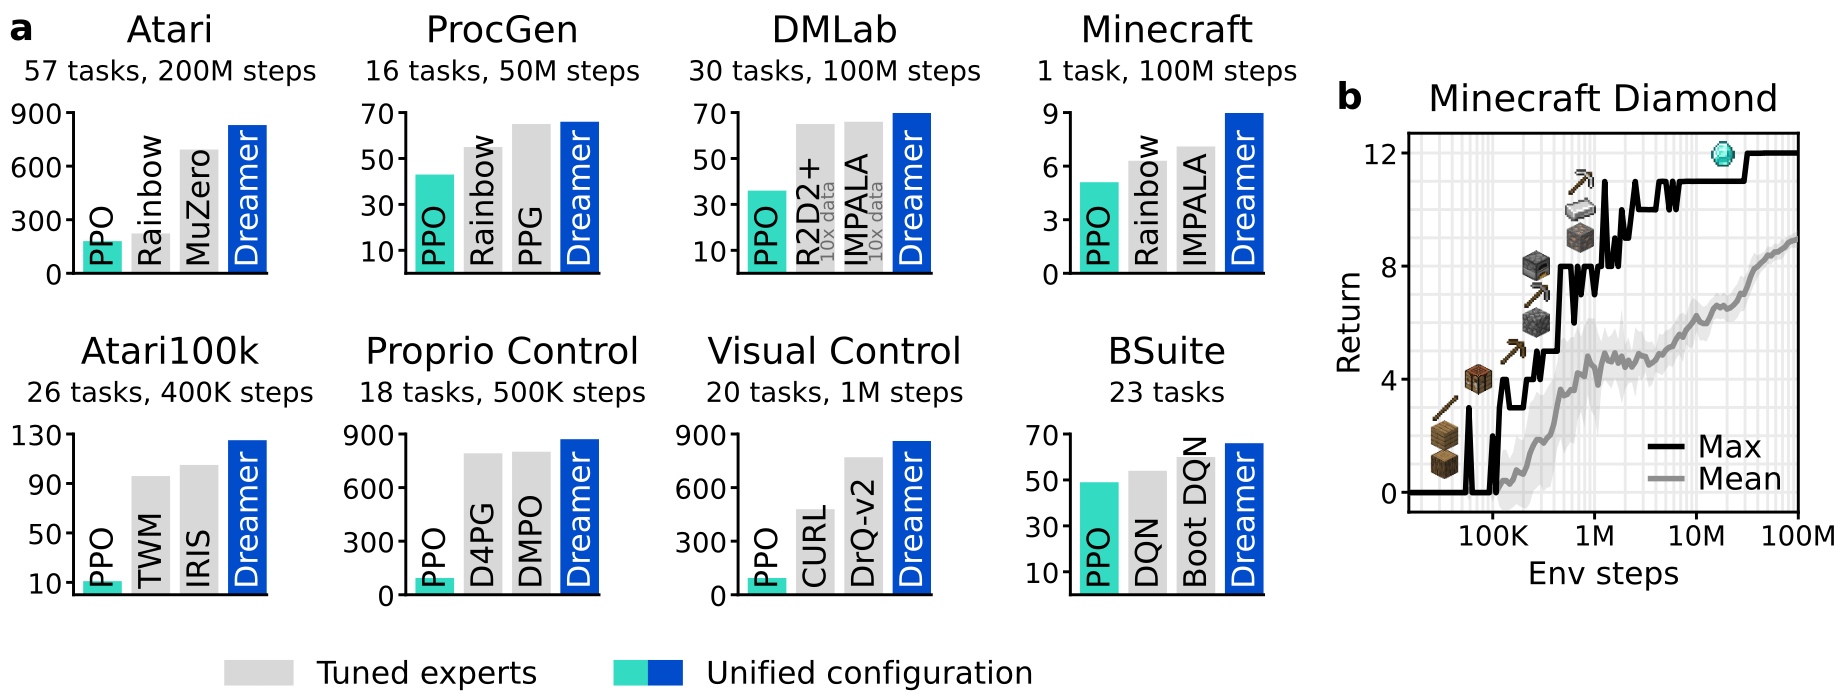
\includegraphics[width=0.7\textwidth]{./pics/benchmarks.png}
    \caption{Summary of benchmark results \cite{hafner2023mastering}}
    \label{fig:results}
\end{figure}

Shortly, DreamerV3 outperforms all the other SOTA algorithms in most of the tasks. The world model also shows its 1) low computation cost, 2) robustness, 3) generalization, 4) data efficiency, 5) scalability, and 6) capability of handling sparse rewards.

\section{Summary of Strengths}

* \textit{The current and following sections are the combination of the author's own understanding with internet reviews. Here I omit the references of these reviews.}

Firstly, the paper is very well organized. The introduction section is clear and concise, providing a good overview of the paper's contributions and significance. The arXiv version of the paper contains over 20 pages of appendices and all the code/results are public accessible in their website. The strict research process and outputs provide a good reference for future research.

Furthermore, the DreamerV3 algorithm is a significant improvement over previous versions and other SOTA algorithms. The use of a world model, actor-critic framework, and the ability to learn from pixels and sparse rewards are impressive. The series of Dreamer algorithms proposes an approach to the problem of model inaccuracy that has plagued researchers in model-base RL for a long time.

Last but not least, the performance of DreamerV3 in not only the Minecraft but also other 150 tasks is really impressive. A reduction in computational cost by several orders of magnitude may very likely make (previously computationally expensive) RL more accessible to researchers and practitioners.

\section{Summary of Weaknesses}

* \textit{I may not be the best person to judge the weaknesses of this paper, but I try my best to summarize some of the weaknesses I found.}

Firstly, the actor-critic framework runs on the latent space, which may cause policy performance limited by the world model accuracy. What's more, the actor-critic framework may still yield out a difficult-to-learn policy in a extremely sparse reward environment. Meanwhile, the algorithm still requires the analysis of explainability, but it is a common challenge in deep RL. The black box nature makes it hard to be well trusted by human users. Lastly, the computation cost of DreamerV3 (specifically in the complex environments like Minecraft) is still need to be improved.

Overall, the series of Dreamer paper are a significant and landmark contribution to the field of reinforcement learning.

\bibliographystyle{unsrtnat}
\bibliography{refs}

\section*{Acknowledgments}
This paper summary was independently conducted by the author Kunyi Yu. Meanwhile, the author would like to thank Professor Jiachen Li and TAs for their patient guidance and help.

\end{document}
